%%%%%%%%%%%%%%%%%%%%%%%%%%%%%%%%%%%%%%%%%%%%%%%%%%%%%%%%%%%%%%%%%%%%%%%%%%%%%%%%
%%%%%%%%%%%%%%%%%%%%%%%%%%%%%%%%%%%%%%%%%%%%%%%%%%%%%%%%%%%%%%%%%%%%%%%%%%%%%%%%
%%                                                                            %%
%% thesistemplate.tex version 3.20 (2018/08/31)                               %%
%% The LaTeX template file to be used with the aaltothesis.sty (version 3.20) %%
%% style file.                                                                %%
%% This package requires pdfx.sty v. 1.5.84 (2017/05/18) or newer.            %%
%%                                                                            %%
%% This is licensed under the terms of the MIT license below.                 %%
%%                                                                            %%
%% Written by Luis R.J. Costa.                                                %%
%% Currently developed at the Learning Services of Aalto University School of %%
%% Electrical Engineering by Luis R.J. Costa since May 2017.                  %%
%%                                                                            %%
%% Copyright 2017-2018, by Luis R.J. Costa, luis.costa@aalto.fi,              %%
%% Copyright 2017-2018 Swedish translations in aaltothesis.cls by Elisabeth   %%
%% Nyberg, elisabeth.nyberg@aalto.fi and Henrik Wallén,                       %%
%% henrik.wallen@aalto.fi.                                                    %%
%% Copyright 2017-2018 Finnish documentation in the template opinnatepohja.tex%%
%% by Perttu Puska, perttu.puska@aalto.fi, and Luis R.J. Costa.               %%
%% Copyright 2018 English template thesistemplate.tex by Luis R.J. Costa.     %%
%% Copyright 2018 Swedish template kandidatarbetsbotten.tex by Henrik Wallen. %%
%%                                                                            %%
%% Permission is hereby granted, free of charge, to any person obtaining a    %%
%% copy of this software and associated documentation files (the "Software"), %%
%% to deal in the Software without restriction, including without limitation  %%
%% the rights to use, copy, modify, merge, publish, distribute, sublicense,   %%
%% and/or sell copies of the Software, and to permit persons to whom the      %%
%% Software is furnished to do so, subject to the following conditions:       %%
%% The above copyright notice and this permission notice shall be included in %%
%% all copies or substantial portions of the Software.                        %%
%% THE SOFTWARE IS PROVIDED "AS IS", WITHOUT WARRANTY OF ANY KIND, EXPRESS OR %%
%% IMPLIED, INCLUDING BUT NOT LIMITED TO THE WARRANTIES OF MERCHANTABILITY,   %%
%% FITNESS FOR A PARTICULAR PURPOSE AND NONINFRINGEMENT. IN NO EVENT SHALL    %%
%% THE AUTHORS OR COPYRIGHT HOLDERS BE LIABLE FOR ANY CLAIM, DAMAGES OR OTHER %%
%% LIABILITY, WHETHER IN AN ACTION OF CONTRACT, TORT OR OTHERWISE, ARISING    %%
%% FROM, OUT OF OR IN CONNECTION WITH THE SOFTWARE OR THE USE OR OTHER        %%
%% DEALINGS IN THE SOFTWARE.                                                  %%
%%                                                                            %%
%%                                                                            %%
%%%%%%%%%%%%%%%%%%%%%%%%%%%%%%%%%%%%%%%%%%%%%%%%%%%%%%%%%%%%%%%%%%%%%%%%%%%%%%%%
%%                                                                            %%
%%                                                                            %%
%% An example for writting your thesis using LaTeX                            %%
%% Original version and development work by Luis Costa, changes to the text   %%
%% in the Finnish template by Perttu Puska.                                   %%
%% Support for Swedish added 15092014                                         %%
%% PDF/A-b support added on 15092017                                          %%
%% PDF/A-2 support added on 24042018                                          %%
%%                                                                            %%
%% This example consists of the files                                         %%
%%         thesistemplate.tex (version 3.20) (for text in English)            %%
%%         opinnaytepohja.tex (version 3.20) (for text in Finnish)            %%
%%         kandidatarbetsbotten.tex (version 1.00) (for text in Swedish)      %%
%%         aaltothesis.cls (versio 3.20)                                      %%
%%         kuva1.eps (graphics file)                                          %%
%%         kuva2.eps (graphics file)                                          %%
%%         kuva1.jpg (graphics file)                                          %%
%%         kuva2.jpg (graphics file)                                          %%
%%         kuva1.png (graphics file)                                          %%
%%         kuva2.png (graphics file)                                          %%
%%         kuva1.pdf (graphics file)                                          %%
%%         kuva2.pdf (graphics file)                                          %%
%%                                                                            %%
%%                                                                            %%
%% Typeset in Linux either with                                               %%
%% pdflatex: (recommended method)                                             %%
%%             $ pdflatex thesistemplate                                      %%
%%             $ pdflatex thesistemplate                                      %%
%%                                                                            %%
%%   The result is the file thesistemplate.pdf that is PDF/A compliant, if    %%
%%   you have chosen the proper \documenclass options (see comments below)    %%
%%   and your included graphics files have no problems.
%%                                                                            %%
%% Or                                                                         %%
%% latex: (this method is not recommended)                                    %%
%%             $ latex thesistemplate                                         %%
%%             $ latex thesistemplate                                         %%
%%                                                                            %%
%%   The result is the file thesistemplate.dvi, which is converted to ps      %%
%%   format as follows:                                                       %%
%%                                                                            %%
%%             $ dvips thesistemplate -o                                      %%
%%                                                                            %%
%%   and then to pdf as follows:                                              %%
%%                                                                            %%
%%             $ ps2pdf thesistemplate.ps                                     %%
%%                                                                            %%
%%   This pdf file is not PDF/A compliant. You must must make it so using,    %%
%%   e.g., Acrobat Pro or PDF-XChange.                                        %%
%%                                                                            %%
%%                                                                            %%
%% Explanatory comments in this example begin with the characters %%, and     %%
%% changes that the user can make with the character %                        %%
%%                                                                            %%
%%%%%%%%%%%%%%%%%%%%%%%%%%%%%%%%%%%%%%%%%%%%%%%%%%%%%%%%%%%%%%%%%%%%%%%%%%%%%%%%
%%%%%%%%%%%%%%%%%%%%%%%%%%%%%%%%%%%%%%%%%%%%%%%%%%%%%%%%%%%%%%%%%%%%%%%%%%%%%%%%

%% USE one of these:
%% * the first when using pdflatex, which directly typesets your document in the
%%   chosen pdf/a format and you want to publish your thesis online,

%% * the second when you want to print your thesis to bind it, or
%% * the third when producing a ps file and a pdf/a from it.
%%
\documentclass[english, 12pt, a4paper, sci, utf8, online]{aaltothesis}
%\documentclass[english, 12pt, a4paper, elec, utf8, a-1b]{aaltothesis}
%\documentclass[english, 12pt, a4paper, elec, dvips, online]{aaltothesis}

%% Use the following options in the \documentclass macro above:
%% your school: arts, biz, chem, elec, eng, sci
%% the character encoding scheme used by your editor: utf8, latin1
%% thesis language: english, finnish, swedish
%% make an archiveable PDF/A-1b or PDF/A-2b compliant file: a-1b, a-2b
%%                    (with pdflatex, a normal pdf containing metadata is
%%                     produced without the a-*b option)
%% typeset in symmetric layout and blue hypertext for online publication: online
%%            (no option is the default, resulting in a wide margin on the
%%             binding side of the page and black hypertext)
%% two-sided printing: twoside (default is one-sided printing)
%%

%% Use one of these if you write in Finnish (see the Finnish template
%% opinnaytepohja.tex)
%\documentclass[finnish, 12pt, a4paper, elec, utf8, a-1b, online]{aaltothesis}
%\documentclass[finnish, 12pt, a4paper, elec, utf8, a-1b]{aaltothesis}
%\documentclass[finnish, 12pt, a4paper, elec, dvips, online]{aaltothesis}

\usepackage{graphicx}

%% Math fonts, symbols, and formatting; these are usually needed
\usepackage{amsfonts,amssymb,amsbsy,amsmath}

%% Change the school field to specify your school if the automatically set name
%% is wrong
% \university{aalto-yliopisto}
% \school{Sähkötekniikan korkeakoulu}

%% Edit to conform to your degree programme
%%
\degreeprogram{Computer, Communication and Information Sciences}
%%

%% Your major
%%
\major{Computer Science}
%%

%% Major subject code
%%
\code{SCI3042}
%%

%% Choose one of the three below
%%
%\univdegree{BSc}
\univdegree{MSc}
%\univdegree{Lic}
%%

%% Your name (self explanatory...)
%%
\thesisauthor{Nikos Heikkilä}
%%

%% Your thesis title comes here and possibly again together with the Finnish or
%% Swedish abstract. Do not hyphenate the title, and avoid writing too long a
%% title. Should LaTeX typeset a long title unsatisfactorily, you mght have to
%% force a linebreak using the \\ control characters.
%% In this case...
%% Remember, the title should not be hyphenated!
%% A possible "and" in the title should not be the last word in the line, it
%% begins the next line.
%% Specify the title again without the linebreak characters in the optional
%% argument in box brackets. This is done because the title is part of the
%% metadata in the pdf/a file, and the metadata cannot contain linebreaks.
%%
\thesistitle{Title of the thesis}
%\thesistitle[Title of the thesis]{Title of\\ the thesis}
%%

%%
\place{Espoo}
%%

%% The date for the bachelor's thesis is the day it is presented
%%
\date{31.8.2018} % TODO change when date known
%%

%% Thesis supervisor
%% Note the "\" character in the title after the period and before the space
%% and the following character string.
%% This is because the period is not the end of a sentence after which a
%% slightly longer space follows, but what is desired is a regular interword
%% space.
%%
\supervisor{Prof.\ Jukka Suomela}
%%

%% Advisor(s)---two at the most---of the thesis. Check with your supervisor how
%% many official advisors you can have.
%%
\advisor{Dr.\ Chetan Gupta}
%\advisor{MSc Sarah Scientist}
%%

%% Aaltologo: syntax:
%% \uselogo{aaltoRed|aaltoBlue|aaltoYellow|aaltoGray|aaltoGrayScale}{?|!|''}
%% The logo language is set to be the same as the thesis language.
%%
\uselogo{aaltoRed}{''}
%%

%% The English abstract:
%% All the details (name, title, etc.) on the abstract page appear as specified
%% above.
%% Thesis keywords:
%% Note! The keywords are separated using the \spc macro
%%
\keywords{For keywords choose\spc concepts that are\spc central to your\spc thesis}
%%

%% The abstract text. This text is included in the metadata of the pdf file as well
%% as the abstract page.
%%
\thesisabstract{
Your abstract in English. Keep the abstract short. The abstract explains your
research topic, the methods you have used, and the results you obtained. In the
PDF/A format of this thesis, in addition to the abstract page, the abstract text is
written into the pdf file's metadata. Write here the text that goes into the
metadata. The metadata cannot contain special characters, linebreak or paragraph
break characters, so these must not be used here. If your abstract does not contain
special characters and it does not require paragraphs, you may take advantage of
the abstracttext macro (see the comment below). Otherwise, the metadata abstract
text must be identical to the text on the abstract page.
}

%% Copyright text. Copyright of a work is with the creator/author of the work
%% regardless of whether the copyright mark is explicitly in the work or not.
%% You may, if you wish, publish your work under a Creative Commons license (see
%% creaticecommons.org), in which case the license text must be visible in the
%% work. Write here the copyright text you want. It is written into the metadata
%% of the pdf file as well.
%% Syntax:
%% \copyrigthtext{metadata text}{text visible on the page}
%%
%% In the macro below, the text written in the metadata must have a \noexpand
%% macro before the \copyright special character, and macros (\copyright and
%% \year here) must be separated by the \ character (space chacter) from the
%% text that follows. The macros in the argument of the \copyrighttext macro
%% automatically insert the year and the author's name. (Note! \ThesisAuthor is
%% an internal macro of the aaltothesis.cls class file).
%% Of course, the same text could have simply been written as
%% \copyrighttext{Copyright \noexpand\copyright\ 2018 Eddie Engineer}
%% {Copyright \copyright{} 2018 Eddie Engineer}
%%
\copyrighttext{Copyright \noexpand\copyright\ \number\year\ \ThesisAuthor}
{Copyright \copyright{} \number\year{} \ThesisAuthor}

%% You can prevent LaTeX from writing into the xmpdata file (it contains all the
%% metadata to be written into the pdf file) by setting the writexmpdata switch
%% to 'false'. This allows you to write the metadata in the correct format
%% directly into the file thesistemplate.xmpdata.
%\setboolean{writexmpdatafile}{false}

% Bibliography
\usepackage[
    backend=bibtex, % TODO change backend
    style=numeric,
    sorting=ynt
]{biblatex}
\addbibresource{refs.bib}

% My extra plugins
\usepackage[textwidth=1in, textsize=footnotesize]{todonotes}
\usepackage[]{tikz}
\usetikzlibrary{positioning,chains,fit,shapes,calc,quotes,matrix}
\usetikzlibrary{arrows.meta,arrows}

\tikzset{main node/.style={circle,fill=blue!20,draw,minimum size=1cm,inner sep=0pt}}
%% All that is printed on paper starts here
%%
\usepackage{caption}
\usepackage{subcaption}

% Commands

% Definitions
\definecolor{myblue}{RGB}{122,152,255}
\definecolor{myorange}{RGB}{255,190,103}

%\DeclareMathOperator{\deg}{deg} % This was already declared

\begin{document}

%% Create the coverpage
%%
\makecoverpage

%% Typeset the copyright text.
%% If you wish, you may leave out the copyright text from the human-readable
%% page of the pdf file. This may seem like a attractive idea for the printed
%% document especially if "Copyright (c) yyyy Eddie Engineer" is the only text
%% on the page. However, the recommendation is to print this copyright text.
%%
\makecopyrightpage

%% Note that when writting your thesis in English, place the English abstract
%% first followed by the possible Finnish or Swedish abstract.

%!tex root = ../main.tex
%% Abstract text
%% All the details (name, title, etc.) on the abstract page appear as specified
%% above.
%%
\begin{abstractpage}[english]
Your abstract in English.
\end{abstractpage}


%% The text in the \thesisabstract macro is stored in the macro \abstractext, so
%% you can use the text metadata abstract directly as follows:
%%
%\begin{abstractpage}[english]
%	\abstracttext{}
%\end{abstractpage}

%% Force a new page so that the possible Finnish or Swedish abstract does not
%% begin on the same page
%%
\newpage

%!tex root = ../main.tex
%%
%% Abstract in Finnish.  Delete if you don't need it.
%%
\thesistitle{Opinnäyteen otsikko}
\supervisor{Prof.\ Jukka Suomela}
\advisor{Dr.\ Chetan Gupta}
%\degreeprogram{Elektroniikka ja sähkötekniikka}
%\department{Elektroniikan ja nanotekniikan laitos}
%\major{Sopiva pääaine}
%% The keywords need not be separated by \spc now.
\keywords{Avainsana1, avainsana2, avainsana3}
%% Abstract text
\begin{abstractpage}[finnish]
  Tiivistelmä tulee tähän.
\end{abstractpage}


%% Force new page so that the Swedish abstract starts from a new page
\newpage

%!tex root = ../main.tex
%% Preface
%%
%% This section is optional. Remove it if you do not want a preface.
\mysection{Preface}
%\mysection{Esipuhe}
I want to thank...\\
\todo{Add thanks}
This work was supported in part by the Academy of Finland, Grant 333837.
\vspace{5cm}
Otaniemi, 31.8.2018

\vspace{5mm}
{\hfill Nikos Heikkilä \hspace{1cm}}


%% Force a new page after the preface
%%
\newpage


%% Table of contents.
%%
\thesistableofcontents


%% Symbols and abbreviations
\mysection{Symbols and abbreviations}

\subsection*{Symbols}

\begin{tabular}{ll}
$c$              & description of this symbol\\
\end{tabular}

\subsection*{Operators}

\begin{tabular}{ll}
$\nabla \times \mathbf{A}$              & description of this operator\\
\end{tabular}

\subsection*{Abbreviations}

\begin{tabular}{ll}
ABC      & multi line description \\
           & for this abbrevation \\
DE        & description for this abbrevation \\
\end{tabular}



%% \clearpage is similar to \newpage, but it also flushes the floats (figures
%% and tables).
%%
\cleardoublepage

\section{Introduction}

The topic of this thesis is related to the field of distributed computing.
It is a field in computer science that studies computation in a distributed fashion.
Distributed computing is any kind of computing that is performed on a spatially distributed system
\cite{DBLP:books/el/leeuwen90/LamportL90}.

Distributed algorithms are designed to solve distributed computing problems.
There are many different problems in distributed computing.
These problems are either possible or impossible to solve.
A problem can be solvable in one distributed computation model and non-solvable in others.
To show that a problem is possible or impossible to solve we need to have a proof.
It can be really tiresome to find proofs manually, therefore it is desirable to develope tools to automate proving.

If a problem is solvable, then there must exist an algorithm that solves the problem in any distributed network.
On the other hand if the problem is impossible to solve, then there exists no algorithm that solves the problem in all distributed networks.
In this work we are interested in the latter case, proving impossibility i.e. proving negative results.

A distributed network is modelled as an undirected graph where each node represents a computer and each edge represents a connection between two computers.
Nodes are always connected to a fixed number of other nodes and the connections do not change.
\cite{DBLP:journals/siamcomp/NaorS95}

An algorithm is the program that is given to each node in the network for execution.
Nodes may also be given different inputs but the programs are identical in every node.
The performance of an algorithm is usually measured by the amount of communication rounds used by the program.
The reason for this is that the nodes have only a limited information available about their neighbourhood and in order to increase this information they will need to communicate.
Communication between nodes takes a considerable amount of time in comparison to the processing capabilities of a node, therefore the reasonable unit of measurement is time in communication rounds. % TODO Write something about synchronised communication between nodes.
Communication round is a synchronised event in which each node can communicate with each of their neighbor.
A node that executes for constant time $t$ has to base its output solely on the information it has gathered from $t$-radius of other nodes
\cite{DBLP:journals/siamcomp/NaorS95}.

Locally checkable labelling (LCL) problems are a family of graph problems for which the validity of a solution can be verified by checking the solution of each node's $\mathcal{O}(1)$-radius neighbourhood (local neighbourhood).
In case all local neighbourhoods are valid, then the whole solution is globally valid.
\cite{DBLP:conf/podc/BrandtHKLOPRSU17}
\footnote{This paragraph does not contain the formal definition of LCL problems.}

Graph coloring is an example of an LCL problem.
In a vertex coloring problem each vertex $v \in V$ of graph $G = (V, E)$ has a label $l(v): V \rightarrow \mathbb{N}$.
The problem itself is that for each $(v, w) \in E$ it must hold that $l(v) \neq l(w)$ i.e. labels must be assigned so that no two adjacent vertices have the same label.
What makes this an LCL problem?
The solution is locally verifiable.
Let the graph represent a distributed network.
Now each node can verify the solution by checking their local neighbourhood of radius 1 and simply check that it does not share a label with any of its neighbors.

Researchers are interested in automating the detection of LCL-problem's constant time solvability in LOCAL model.
There already exists a tool called \emph{round eliminator} \cite{DBLP:conf/podc/Olivetti20} which uses a \emph{round elimination} \cite{DBLP:conf/podc/Brandt19} technique to automatically find lower bounds of LCL problems.
Round eliminator can tell if an LCL problem is solvable in constant time and this can be done fairly fast if the constant is small (as far as I know).
There can be multiple reasons for a LCL problem to not be solvable in constant time.
One such reason is that the problem is not solvable in PN (port number) model
\footnote{Some how there is a connection between constant time solvability in LOCAL model and solvability in PN model.}.
We would like to detect this particular case.


\subsection*{Objective} % TODO Change to 'Objectives' and explain all of the objectives.
The objective is to develope a tool (computer program) which tells if an LCL (locally checkable labelling) problem is not solvable in PN (port number) model.
The idea is to find a network where there exists no valid labellings implying that the problem is impossible to solve.
The tool should work fast, therefore optimizations are one of the main focuses of the work.

At first the tool will have a command line interface.
Later on the tool is planned to have a browser user interface.

The input should be given in the same format as the Round eliminator uses to represent LCL problems.
This is important because we can use the same input format in both tools.

Preferably the proof of non-solvability of the problem should be visualized.
This can be done for example by rendering the network that cannot have any viable configurations.


%% Leave page number of the first page empty
%%
\thispagestyle{empty}

\clearpage
%!tex root = ../main.tex
%% Background
%%
\section{Background}
\todo{Could also be named as "Theoretical background"}
To understand the implementation chapter \ref{sec:solution}, in this section we introduce relevant terminology and concepts.

\todo{Add info about section \ref{sec:graphs}}

In the first section (\ref{sec:distributed_computing}) of this chapter, we discuss about the essential concepts in the theory of distributed computing.
The section aims to explain the meaning of distributed computing and gives an introduction to the main model of distributed computing, \emph{message passing model}, from which many of the researched models inherit from.

The second and third sections discuss about the Port number model and local model respectively.
These are widely used models in the field and they are strongly related to the research showed in this paper.

We are trying to find lower bound proofs for LCL-problems in this paper, therefore it is essential to include a section entirely for them.
The fourth section (\ref{sec:lcl_problems}) is dedicated to LCL-problems.

Finally, in the last section (\ref{sec:previous_research}), we talk about previous research in the field and research that are more related to this thesis.

\subsection{Graphs} \label{sec:graphs}
In the real world, there are many objects that are somehow related to each other.
Such things can often be visualized by a diagrams that consists of points, and lines that connect a pair of points.
A graph is a mathematical concept that abstracts the relations of these objects.
In the literature, the points are called vertices and lines are called edges.
\cite{DBLP:books/others/BondyM76}

Mathematically, graph can be defined as a tuple $$G = (V, E)$$ where $V$ is the set of vertices and $E$ is the set of edges.
%Each vertex $v \in V$
Each edge $e \in E$ can also be thought as a tuple $e=(v, w), v, w \in V$, where vertices $v$ and $w$ are the endpoints of the edge $e$.
For example, $G=(\{1, 2, 3\}, \{(1, 2),(1, 3),(2, 3),(3, 2)\})$, and visualized it looks like the graph on figure \ref{fig:graph1:a}.

When the order of the vertices in an edge matters, we call the graph as a \emph{directed graph} or with the shortened variation \emph{digraph}.
For digraphs, the following statement must hold:
\begin{equation} \label{eq:1}
\forall v, w \in V, v \neq w: (v, w) \neq (w, v)
\end{equation}
In that case, the first vertex $v$ points to the vertex $w$.
Usually the edge is visualized as an arrow pointing from $v$ to $w$.
One example of a directed graph is a flow graph, in which the edges represent flows from a vertex to another vertex, as seen in the figure \ref{fig:graph1:a}.

\begin{figure}[h]
  \subcaptionbox{A simple directed graph.\label{fig:graph1:a}}%
    [.3\linewidth] {
    \centering
    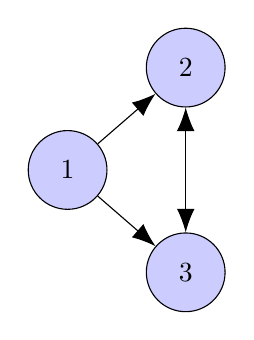
\begin{tikzpicture}[>={Latex[length=3mm]},auto, on grid, ]
      \node[main node] (1) {$1$};
      \node[main node] (2) [above right = 1.3cm and 1.5cm of 1] {$2$};
      \node[main node] (3) [below right = 1.3cm and 1.5cm of 1] {$3$};
      \draw[->] (1) edge[] node {} (2);
      \draw[->] (1) edge[] node {} (3);
      \draw[<->] (2) edge[] node {} (3);
    \end{tikzpicture}
  }
  \hfill
  \subcaptionbox{A simple undirected graph.\label{fig:graph1:b}}%
    [.3\linewidth] {
    \centering
    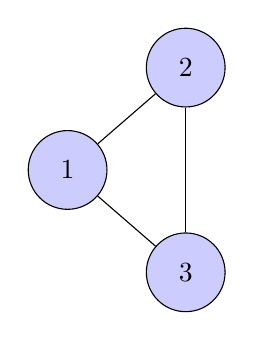
\begin{tikzpicture}[auto, on grid, ]
      \node[main node] (1) {$1$};
      \node[main node] (2) [above right = 1.3cm and 1.5cm of 1] {$2$};
      \node[main node] (3) [below right = 1.3cm and 1.5cm of 1] {$3$};
      \draw[-] (1) edge[] node {} (2);
      \draw[-] (1) edge[] node {} (3);
      \draw[-] (2) edge[] node {} (3);
    \end{tikzpicture}
  }
  \hfill
  \subcaptionbox{An undirected multigraph.\label{fig:graph1:b}}%
    [.3\linewidth] {
    \centering
    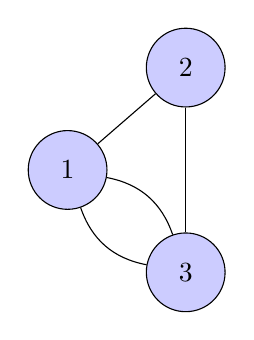
\begin{tikzpicture}[auto, on grid, ]
      \node[main node] (1) {$1$};
      \node[main node] (2) [above right = 1.3cm and 1.5cm of 1] {$2$};
      \node[main node] (3) [below right = 1.3cm and 1.5cm of 1] {$3$};
      \draw[-] (1) edge[] node {} (2);
      \draw[-] (1) edge[bend left] node {} (3);
      \draw[-] (1) edge[bend right] node {} (3);
      \draw[-] (2) edge[] node {} (3);
    \end{tikzpicture}
  }
  \caption{Examples of different graphs}
  \label{fig:graph1}
\end{figure}

\todo{refer the figures from the text and fix old refers}

Undirected graph is the opposite of directed graph in the sense that the order of the vertices in an edge does not matter:
\begin{equation}
\forall v, w \in V: (v, w) = (w, v)
\end{equation}
For example $E=\{(1, 2), (1, 2), (3, 2), (2, 3), (1, 3)\}=\{(1,2),(1,3),(2,3)\}$.
Visualization of this graph can be seen in the figure \ref{fig:graph1:b}.
For the purpose of this work, we need only undirected edges.

The definitions of graphs shown earlier do not restrict an edge to start and end in itself ($e=(v, v)$).
This kind of an edge is called a \emph{loop}.
The definition however restricts multiple same edges, \emph{parallel edges}.
In order to allow parallel edges, the edge set has to be defined as a multiset.
A graph that allows parallel edges, is called a \emph{multigraph}.
Depending on the author or context, multigraphs either allow or disallow loops.
In this work, we consider multigraphs to exist without loops.
Notice that on the figure \ref{fig:graph1:a}, there is an edge that points to both directions.
This is, in fact, not one but two edges in parallel.
It is common to visualize such cases using a two-way arrow.

A graph that has no loops or parallel edges, is called as a \emph{simple graph}.
Simple graphs can either be directed or undirected and it should be explicitly mentioned when defining graphs, unless the context implies it.
As we do not need directedness of edges, let us assume that further expressions of graphs are always undirected.

For an edge $e=(v, w) \in E$ we say that $v$ is \emph{incident} to $w$ and vice versa.
If two edges share a vertex, we say that the edges are \emph{adjacent}.
The degree of a vertex is the number of edges it is connected to.
We will use the notation $\deg_G(v)$ to denote the degree of vertex $v \in V, G=(V,E)$.

A graph that is bipartite, has exactly two disjoint sets of vertices ($A$ and $B$), and every edge of the graph has one endpoint in vertex of $A$ and another in $B$:
\begin{equation}
V = A \cup B, A \cap B = \emptyset, E=\{(a, b) | a \in A, b \in B\}
\end{equation}
For bipartite graphs, the sum of degrees on A and B are equal:
\begin{equation}
\sum_{a\in A} \deg_G(a) = \sum_{b\in B} \deg_G(b)
\end{equation}
An example of a bipartite graph can be seen in the figure \ref{fig:graph2}.

\begin{figure}[h]
\centering
% https://tex.stackexchange.com/a/499577
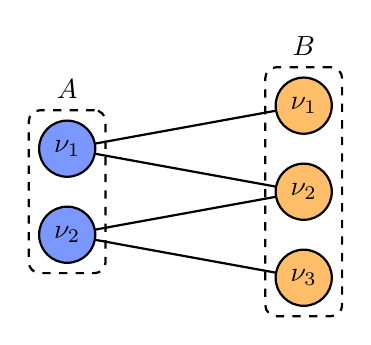
\begin{tikzpicture}[thick,amat/.style={matrix of nodes,nodes in empty cells,
  row sep=1em,draw,dashed,rounded corners,
  nodes={draw,solid,circle,execute at begin node={$\nu_{\the\pgfmatrixcurrentrow}$}}},
  fsnode/.style={fill=myblue},
  ssnode/.style={fill=myorange}]

  \matrix[amat,nodes=fsnode,label=above:$A$] (mat1) {\\
  \\};

  \matrix[amat,right=2cm of mat1,nodes=ssnode,label=above:$B$] (mat2) {\\
  \\
  \\};

  \draw  (mat1-1-1) edge (mat2-1-1);
  \draw (mat1-1-1) edge (mat2-2-1);
  \draw (mat1-2-1) edge (mat2-2-1);
  \draw (mat1-2-1) edge (mat2-3-1);
\end{tikzpicture}
\caption{A simple bipartite graph.\label{fig:graph2}}
\end{figure}


\newpage
\subsection{Distributed computing} \label{sec:distributed_computing}
Computing or processing a computer program in several identical or different computation nodes is called distributed computing.
It is similiar to running a computer program that contains multiple concurrent tasks, but in distributed computing there are higher level tasks that are distributed to different computer nodes.

Computation nodes are connected to each others with communication channels.
These communication channels carry data from node to another node.
Together, nodes and communication channels form a network.
The best way to visualize these networks is by drawing a graph in which the nodes represent computing nodes and edges represent the communication channels.

\begin{figure}[h]
  \centering
  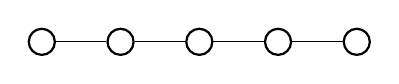
\begin{tikzpicture}[every node/.style={circle,thick,draw}]
  \node (1) {};
  \node (2) [ right of=1] {};
  \node (3) [ right of=2] {};
  \node (4) [ right of=3] {};
  \node (5) [ right of=4] {};
  \draw (1) -- (2);
  \draw (2) -- (3);
  \draw (3) -- (4);
  \draw (4) -- (5);
\end{tikzpicture}
\caption{Example of a distributed network.}
\label{fig:dist_comp_1}
\end{figure}

According to Lamport \cite{DBLP:books/el/leeuwen90/LamportL90}, in the area of distributed computing, the term \emph{model} denotes a view or abstract representation of a distributed system.
There are multiple different computation models used in distributed computing.
The most important main category of distributed computation models is \emph{process models}.
In process models, the work or activities are represented as concurrently executed processes that execute their instructions sequentially.
The main way to distinguish different process models from each other is to categorise them by the method they use to communicate with each other (\emph{interprocess communication}).
\cite{DBLP:books/el/leeuwen90/LamportL90}

Message passing models are a form of process model.
They are widely researched, for example ... \todo{add references to papers that research or use message passing models}
In the model, processes communicate by adding a message to message queue, wheter it is a shared or a process specific, and the recipient process removes the message (dequeues) from the message queue.
\cite{DBLP:books/el/leeuwen90/LamportL90}


%The following two sections (\ref{sec:port_number_model} and \ref{sec:local_model} ) talk about different forms of message passing models that are highly relative to this paper.

%In the theory of distributed computing, it is common to use terminology and concepts from graph theory as networks are basically graphs.
%With formal definitions, we can discuss more about the structure of distributed networks and reason features of those networks.
%We can further construct proofs of different theorems and so on. \todo{Fix this paragraph}

The algorithms that are executed in distributed fashion, are called distributed algorithms. \todo{where to write about distributed algorithms?}
%A distributed algorithm is a specific type of algorithm that is executed in distributed fashion.
Specifically, each node executes the same algorithm.

\todo{write about computation models, why they exist}
\todo{Add message passing model before PN model}
\subsubsection{Message passing model} \label{sec:message_passing_model}
\subsubsection{Port Number model} \label{sec:port_number_model}
\subsubsection{LOCAL model} \label{sec:local_model}
\subsection{LCL problems} \label{sec:lcl_problems}
\subsection{Previous research} \label{sec:previous_research}
\todo{Especially LCL classification research}
\clearpage


\section{Research material and methods}
\todo{Under the methods, I can write about software development methods used. Remember that }
\clearpage

\section{Automatically proving lower bounds for LCL problems} \label{sec:solution}
\todo{TODO should this title be just "Implementation"? Probably.}
\subsection{Generating LCL-problems}
\subsection{Generating graphs}
\subsection{SAT encoding and solving}
\subsection{Software optimizations}

\clearpage

\section{Results} \label{sec:results}
\todo{Show all results that have been found while doing the research, like different problems that have now new lower bounds.}

\clearpage

\section{Summary} \label{sec:summary}

\clearpage

\thesisbibliography
\printbibliography


\clearpage

\thesisappendix

\section{First example appendix\label{AppendixA}}

\clearpage
\section{Second example appendix\label{AppendixB}}


\end{document}
